\begin{figure}[h]
    \centering
    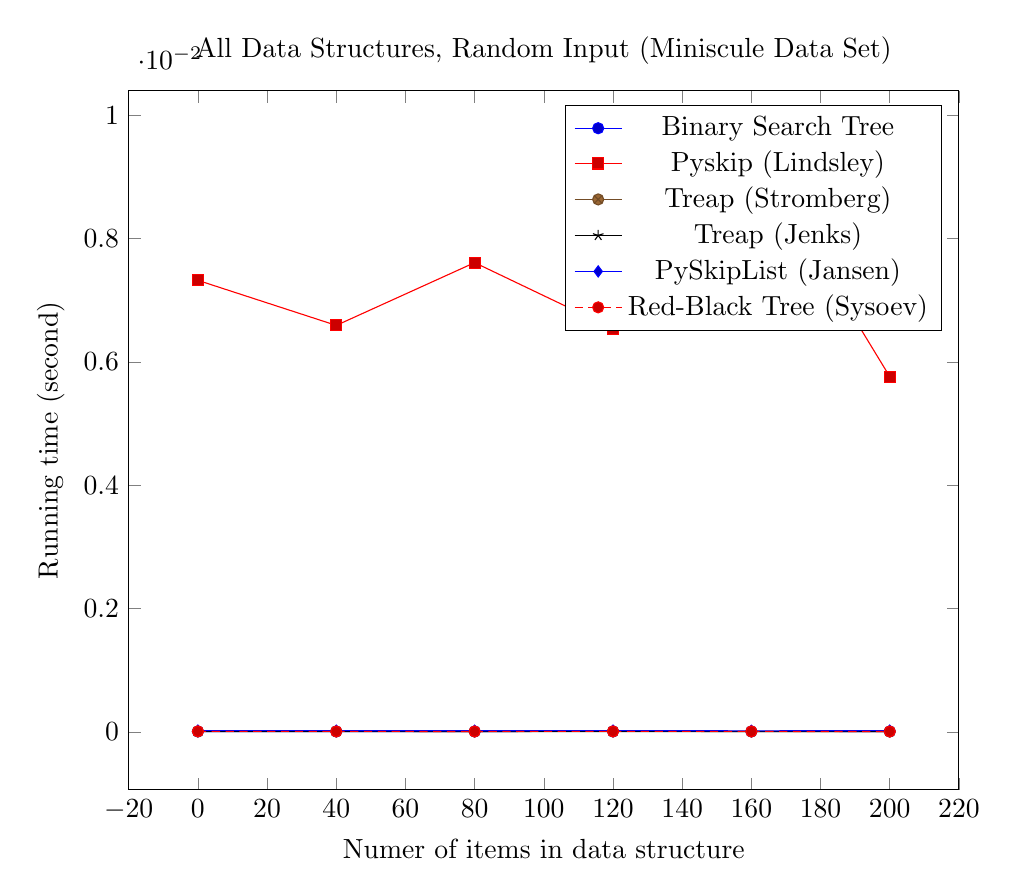
\begin{tikzpicture}
        \begin{axis}[
            xlabel={Numer of items in data structure},
            ylabel={Running time (second)},
            title={All Data Structures, Random Input (Miniscule Data Set)},
            width=\textwidth
        ]
		\addplot coordinates {
			(0, 5.330803460523726e-06)
			(40, 5.330803460523726e-06)
			(80, 5.3308034604349075e-06)
			(120, 5.722331398239078e-06)
			(160, 5.511508662525699e-06)
			(200, 5.421156061480304e-06)
		};
		\addplot coordinates {
			(0, 0.0073206689104229564)
			(40, 0.006590107896064445)
			(80, 0.007607929946616654)
			(120, 0.006535083162039879)
			(160, 0.009447629373630662)
			(200, 0.00575952655237062)
		};
		\addplot coordinates {
			(0, 5.481391128903112e-06)
			(40, 6.0536242687092566e-06)
			(80, 4.96939305643096e-06)
			(120, 6.143976869754653e-06)
			(160, 5.059745657476355e-06)
			(200, 4.547747584915385e-06)
		};
		\addplot coordinates {
			(0, 2.8009306317855477e-06)
			(40, 2.349167626647386e-06)
			(80, 2.108227357222603e-06)
			(120, 2.3190500929359813e-06)
			(160, 2.108227357222603e-06)
			(200, 2.1383448909340075e-06)
		};
		\addplot coordinates {
			(0, 1.9455926754208262e-05)
			(40, 1.7799462401946187e-05)
			(80, 1.6534525987665916e-05)
			(120, 1.8883693614313302e-05)
			(160, 1.5269589573296825e-05)
			(200, 1.828134294088457e-05)
		};
		\addplot coordinates {
			(0, 7.017385346230754e-06)
			(40, 5.541626196237104e-06)
			(80, 5.391038527768899e-06)
			(120, 6.143976869754653e-06)
			(160, 5.692213864616491e-06)
			(200, 4.909157989096969e-06)
		};
        \legend{Binary Search Tree, Pyskip (Lindsley), Treap (Stromberg), Treap (Jenks), PySkipList (Jansen), Red-Black Tree (Sysoev)}
        \end{axis}
    \end{tikzpicture}
    \caption{Average of 10 operations, benchmarked every 40, starting at 0.}
\end{figure}